% Unit 106 terjemahan Bahasa Indonesia dari chapter8.tex baris 1--174.
% Sumber: Methods of Algebra, Volume 2, commit
% 9a5803ff77dd3257484cb177f851a73770a59dd3 (CC BY 4.0).
% stable-unit-id: o014.aljabr2.chapter8.simplicial-objects
% Cakupan: pembukaan Bab 8 dan Bagian 8.1 lengkap;
% berhenti tepat sebelum Bagian 8.2 pada baris 175.

% Sumber asli: Copyright 2024 李文威 (Wen-Wei Li), CC BY 4.0.

% segment-id: o014.li2.chapter8.simplicial-objects.h001
\chapter{Metode Simplisial}\label{sec:simplicial}
\hypertarget{o014.aljabr2.chapter8.simplicial-objects}{ }
% segment-id: o014.li2.chapter8.simplicial-objects.p001
Misalkan $\simpDelta$ kategori ordinal hingga tak kosong. Menurut definisi,
objek simplisial dalam kategori $\mathcal{C}$ adalah funktor
$X:\simpDelta^{\opp}\to\mathcal{C}$. Secara ekuivalen, objek ini dapat
dideskripsikan sebagai deretan objek $X_0,X_1,\ldots$ beserta morfisme
$d_i:X_n\to X_{n-1}$ (muka) dan $s_j:X_n\to X_{n+1}$ (degenerasi), untuk
$0\leq i,j\leq n$, yang memenuhi keluarga identitas
\eqref{eqn:simplicial-identity}. Funktor-funktor tersebut membentuk kategori
$\cate{s}\mathcal{C}$. Dalam kasus khusus $\mathcal{C}=\cate{Set}$,
objek-objek ini juga disebut himpunan simplisial. Teori dasarnya dibahas
dalam \S\S\ref{sec:simplicial-method}--\ref{sec:simplicial-set}. Tuliskan
$\cate{FinOrd}$ untuk kategori ordinal hingga. Jika objek simplisial $X$,
sebagai funktor, meluas menjadi funktor $\cate{FinOrd}\to\mathcal{C}$, maka
$X$ disebut objek simplisial teraugmentasi. Hal ini sama artinya dengan
menambahkan suku berderajat $-1$, $X_{-1}$, pada data
$(X_n,d_i,s_j)_{n,i,j}$.

% segment-id: o014.li2.chapter8.simplicial-objects.p002
Himpunan simplisial berasal dari topologi. Gagasan dasarnya ialah menguraikan
ruang sebagai hasil penempelan simpleks; gambaran intuitif simpleks (titik, ruas garis,
segitiga, tetrahedron, dan seterusnya) adalah
% segment-id: o014.li2.chapter8.simplicial-objects.g001
\begin{center}\begin{tabular}{ccccc}
	$0$ dimensi & $1$ dimensi & $2$ dimensi & $3$ dimensi & $\cdots$ \\
	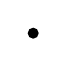
\begin{tikzpicture}[baseline=(P)] \fill[black] (0.5, 0.5) circle[radius=0.07]; \coordinate (P) at (0, 0.5); \end{tikzpicture} &
	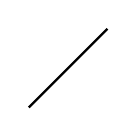
\begin{tikzpicture}[baseline=(P)] \draw[thick] (0,0) -- (1,1); \coordinate (P) at (0.5, 0.5); \end{tikzpicture} &
	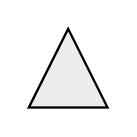
\begin{tikzpicture}[baseline=(P)] \filldraw[thick, fill=gray!15] (0,1) -- (-0.5, 0) -- (0.5, 0) --cycle; \coordinate (P) at (0, 0.5); \end{tikzpicture} &
	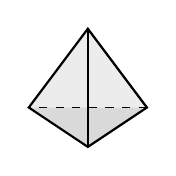
\begin{tikzpicture}[baseline=(P)]
		\fill[color=gray!15] (0, 1) -- (0.75, 0) -- (0, -0.5) -- (-0.75, 0) --cycle;
		\fill[color=gray!30] (0.75, 0) -- (0, -0.5) -- (-0.75, 0) --cycle;
		\draw[dashed] (0.75, 0) -- (-0.75, 0);
		\draw[thick] (0, 1) -- (0.75, 0) -- (0, -0.5) -- (-0.75, 0) --cycle;
		\draw[thick] (0, 1) -- (0, -0.5);
		\coordinate (P) at (0, 0.3);
	\end{tikzpicture} &
	$\cdots$
\end{tabular}\end{center}
Penguraian tersebut memberikan cara konkret dan kombinatorial untuk memahami
homologi, homotopi, dan persoalan lain mengenai ruang. Rumusan ketat yang
digunakan di sini diperkenalkan oleh S.\ Eilenberg dan J.\ A.\ Zilber pada
1950. Bahasa himpunan simplisial memiliki jangkauan luas dan tidak terbatas
pada persoalan topologi klasik. Sebagai contoh, bahasa ini dapat
mendeskripsikan kategori melalui konstruksi yang disebut ``saraf'', yang
diperkenalkan dalam \S\ref{sec:nerves}. Teori kategori membahas objek dalam
diagram (ditampilkan sebagai titik berdimensi nol), morfisme (ditampilkan
sebagai anak panah berdimensi satu), dan komutativitas (yang berkaitan dengan
komponen berdimensi dua seperti segitiga atau persegi). Jadi, tidak
mengherankan bahwa kategori dan ruang dapat dipadukan dalam struktur
matematis yang sama.

% segment-id: o014.li2.chapter8.simplicial-objects.p003
Setelah saraf dan ruang klasifikasi diperkenalkan sebagai contoh dasar
himpunan simplisial, \S\ref{sec:geom-realization} kembali pada intuisi dan
mendefinisikan realisasi geometris $|X|$ dari himpunan simplisial $X$.
Teorema~\ref{prop:geom-Sing-adjunction} menunjukkan bahwa realisasi geometris
bersama funktor himpunan singular $\mathrm{Sing}$ yang dikenal dalam topologi
membentuk pasangan adjoin
% segment-id: o014.li2.chapter8.simplicial-objects.q001
\[\begin{tikzcd}
	{|\cdot|}: \cate{sSet} \arrow[shift left, r] & \cate{Top} : \mathrm{Sing}. \arrow[shift left, l]
\end{tikzcd}\]
Jika $\cate{Top}$ diganti dengan kategori ruang Hausdorff yang dibangkitkan
secara kompak, $\cate{CGHaus}$, yang lazim dalam teori homotopi, realisasi
geometris juga memenuhi $|X\times Y|\simeq|X|\times|Y|$. Produk pada ruas
kiri dibentuk suku demi suku dari kedua himpunan simplisial. Buktinya berkaitan
dengan triangulasi produk dan melibatkan beberapa rincian kombinatorial yang
tidak sepele; karena buku ini bukan buku teks topologi, rincian tersebut tidak
dibahas lebih jauh.

% segment-id: o014.li2.chapter8.simplicial-objects.p004
Untuk tema buku ini, yang lebih penting ialah objek simplisial dalam kategori
abelian $\mathcal{A}$. Dalam keadaan ini, $\cate{s}\mathcal{A}$ juga kategori
abelian; sebagai contoh, grup abelian simplisial membentuk kategori abelian
$\cate{sAb}$. Hasil dasarnya adalah korespondensi Dold--Kan dalam
\S\ref{sec:Dold-Kan} (Teorema~\ref{prop:Dold-Kan}), yang untuk kategori abelian
$\mathcal{A}$ memberikan pasangan ekuivalensi adjoin
% segment-id: o014.li2.chapter8.simplicial-objects.q002
\[\begin{tikzcd}
	\Gamma: \cate{s}\mathcal{A} \arrow[shift left, r] & \cate{Ch}_{\geq 0}(\mathcal{A}): \mathrm{N}, \arrow[shift left, l]
\end{tikzcd}\]
dengan $\cate{Ch}_{\geq0}(\mathcal{A})$ menyatakan kategori abelian kompleks rantai
berderajat nonnegatif di atas $\mathcal{A}$. Funktor $\mathrm{N}$ memetakan
objek simplisial $X$ ke kompleks rantai ternormalisasi $\mathrm{N}X$ yang
bersesuaian. Lebih tepatnya, definisikan kompleks rantai tak ternormalisasi
dari $X\in\Obj(\cate{s}\mathcal{A})$ sebagai
% segment-id: o014.li2.chapter8.simplicial-objects.q003
\[ \mathrm{C}X := \left( X_n, \partial_n\right)_{n \geq 0}, \quad \partial_n := \sum_{i=0}^n (-1)^i d_i : X_n \to X_{n-1}. \]
Maka $\mathrm{N}X$ dapat diambil sebagai subkompleks rantai dari
$\mathrm{C}X$ melalui
$(\mathrm{N}X)_n:=\bigcap_{i=1}^n\Ker(d_i)$, atau dipandang sebagai hasil
bagi $\mathrm{C}X$ oleh bagian degenerat. Isomorfisme antara kedua bentuk ini
adalah isi Proposisi~\ref{prop:Dold-Kan-v}. Bahkan,
Teorema~\ref{prop:Dold-Kan-N-C} menunjukkan bahwa morfisme inklusi
$u:\mathrm{N}X\to\mathrm{C}X$ adalah kuasi-isomorfisme antarkompleks rantai.

% segment-id: o014.li2.chapter8.simplicial-objects.p005
Korespondensi Dold--Kan menjadikan teori simplisial salah satu sumber
aljabar homologis, bukan hanya secara historis, melainkan juga secara konseptual
dan teknis. Metode simplisial dapat menjelaskan dan memperkaya operasi
dasar pada kompleks atau kompleks rantai; misalnya, homotopi dan
kontraktibilitas mempunyai versi simplisial sehingga memperoleh
interpretasi topologis. Hal ini dibahas dalam
\S\ref{sec:homology-computation}.

% segment-id: o014.li2.chapter8.simplicial-objects.p006
Penerapan lain menghubungkannya dengan teori monad dari \S\ref{sec:Beck}.
Dengan cara ini, objek suatu kategori dapat diperluas secara kanonik menjadi objek simplisial
teraugmentasi atau objek kosimplisial teraugmentasi. Karena berkaitan dengan
operasi ``menambahkan bar'' dalam homologi Hochschild, teknik-teknik tersebut
secara kolektif disebut konstruksi bar dan menjadi tema
\S\ref{sec:bar-resolution}. Melalui korespondensi Dold--Kan dan beberapa
pengamatan tentang sifat dapat dikontraksi, konstruksi bar menjelaskan
berbagai resolusi standar dalam teori Hochschild (lihat \S\ref{sec:HH}) dan
teori kohomologi grup (lihat \S\ref{sec:G-mod}); semuanya ternyata berasal
dari satu gagasan pada aras yang lebih tinggi. Latihan memuat perluasan lain tentang
konstruksi bar.

% segment-id: o014.li2.chapter8.simplicial-objects.p007
Menurut definisi, objek bisimplisial yang dibahas dalam
\S\ref{sec:bisimplicial} tidak lain adalah funktor
$\simpDelta^{\opp}\times\simpDelta^{\opp}\to\mathcal{C}$; semuanya membentuk
kategori $\cate{s}^2\mathcal{C}$. Bila $\mathcal{A}$ kategori abelian, Teorema
Eilenberg--Zilber~\ref{prop:Eilenberg-Zilber}, yang langsung berkaitan dengan
$\cate{s}^2\mathcal{A}$, merupakan konstruksi dasar dalam topologi aljabar.
Dari sudut pandang teori kategori murni, bila $\mathcal{A}$ kategori monoidal
(misalnya $\mathcal{A}=\cate{Ab}$), teorema itu memberikan dua struktur monoidal
kanonik, dengan arah yang berlawanan, pada funktor
$\mathrm{N}:\cate{s}\mathcal{A}\to\cate{Ch}_{\geq0}(\mathcal{A})$. Namun,
penerapan objek bisimplisial tidak terbatas pada hal ini.

% segment-id: o014.li2.chapter8.simplicial-objects.p008
Dua bagian terakhir bab ini, \S\ref{sec:closed-simplicial} dan
\S\ref{sec:mapping-cone-revisited}, masing-masing membahas objek $\Hom$ dan
kerucut pemetaan bagi himpunan simplisial. Di satu sisi, keduanya
bersesuaian dengan ruang pemetaan dan kerucut menurut intuisi topologis. Di sisi
lain, pada kasus grup abelian, melalui korespondensi Dold--Kan, keduanya
memberikan kompleks rantai $\Hom$ dan kerucut pemetaan yang dikenal. Jadi,
konstruksi terkait pada kompleks atau kompleks rantai memperoleh penjelasan
yang jernih, sedangkan bagi topolog semua ini sudah sangat akrab.

% segment-id: o014.li2.chapter8.simplicial-objects.n001
\begin{wenxintishi}
	Bagian \S\S\ref{sec:simplicial-method}--\ref{sec:geom-realization}
	membentuk tulang punggung metode simplisial dalam bab ini;
	\S\S\ref{sec:Dold-Kan}--\ref{sec:bar-resolution} berhubungan langsung
	dengan kompleks rantai; dan walaupun
	\S\S\ref{sec:bisimplicial}--\ref{sec:mapping-cone-revisited} selaras dengan
	isi buku sebelumnya, bagian-bagian ini lebih bersifat lanjutan. Dibandingkan
	bab-bab lain, metode simplisial tidak diperlukan secara logis. Namun,
	gagasan dan tekniknya termasuk bekal dasar bagi matematikawan dan menjadi
	landasan untuk memasuki aljabar tingkat lanjut. Sebagian argumen tentang
	objek simplisial kadang-kadang melibatkan pemeriksaan rutin yang panjang
	(seperti dalam \S\ref{sec:Dold-Kan}); hal ini merupakan konsekuensi
	definisinya, dan pembaca dapat menentukan sendiri seberapa jauh hendak
	menelusurinya.
\end{wenxintishi}

% segment-id: o014.li2.chapter8.simplicial-objects.h002
\section{Objek Simplisial}\label{sec:simplicial-method}
% segment-id: o014.li2.chapter8.simplicial-objects.p009
Dalam Catatan~\ref{rem:walking-algebra}, kita mengingat kembali pemetaan
monoton antara himpunan terurut parsial dan menggunakannya untuk mendefinisikan
kategori ordinal hingga $\cate{FinOrd}$. Bab ini berfokus pada subkategori
penuh $\simpDelta$ yang terdiri atas ordinal tak kosong.

% segment-id: o014.li2.chapter8.simplicial-objects.d001
\begin{definition}
	\index[sym1]{Delta-simp@$\simpDelta$}
	\index[sym1]{[n]}
	Misalkan $\simpDelta$ kategori semua ordinal hingga tak kosong dan
	pemetaan monoton di antaranya. Dengan kata lain, objeknya adalah himpunan
	terurut total $[n]:=\{0,\ldots,n\}$ untuk $n\in\Z_{\geq0}$ dan
	morfismenya pemetaan monoton.
\end{definition}

% segment-id: o014.li2.chapter8.simplicial-objects.p010
Perhatikan bahwa $[n]$ tidak boleh dikacaukan dengan $\mathbf{n}$, yang dalam
buku ini menyatakan himpunan terurut total $\{0,\ldots,n-1\}$ atau kategori
yang bersesuaian.

% segment-id: o014.li2.chapter8.simplicial-objects.p011
Setiap morfisme $[l]\to[n]$ dalam $\simpDelta$ mempunyai faktorisasi unik
sebagai komposisi suatu pemetaan monoton surjektif dan pemetaan monoton
injektif,
% segment-id: o014.li2.chapter8.simplicial-objects.q004
\[ [l] \twoheadrightarrow [m] \hookrightarrow [n], \quad n \geq m \leq l. \]
Pemetaan injektif (atau surjektif) seperti di atas dapat diuraikan lebih lanjut
menjadi potongan-potongan yang pada setiap langkah tepat melewatkan satu
elemen (atau tepat mengidentifikasi dua elemen). Dengan kata lain, semua
morfisme dapat difaktorkan menjadi komposisi dua jenis morfisme berikut.
% segment-id: o014.li2.chapter8.simplicial-objects.q005
\begin{center}\begin{tabular}{|c|l|l|l|} \hline
	Komuka & $\mathrm{d}^i = \mathrm{d}^{n, i}: [n-1] \hookrightarrow [n]$ & $0 \leq i \leq n$ & injeksi monoton yang hanya melewatkan $i\in[n]$ \\ \hline
	Kodegenerasi & $\mathrm{s}^j = \mathrm{s}^{n, j}: [n+1] \twoheadrightarrow [n]$ & $0 \leq j \leq n$ & surjeksi monoton yang mengambil $j\in[n]$ dua kali \\ \hline
\end{tabular}\end{center}

% segment-id: o014.li2.chapter8.simplicial-objects.p012
Suatu pemetaan monoton injektif (atau surjektif) dapat diuraikan menjadi
komuka (atau kodegenerasi) dengan beberapa cara, bergantung pada urutan
elemen yang dilewatkan (atau diidentifikasi). \emph{Identitas kosimplisial}
berikut mudah diperiksa:
% segment-id: o014.li2.chapter8.simplicial-objects.q006
\begin{equation}\label{eqn:cosimplicial-identity}\begin{array}{ll}
	\mathrm{d}^j \mathrm{d}^i = \mathrm{d}^i \mathrm{d}^{j-1}, & i < j, \\
	\mathrm{s}^j \mathrm{d}^i = \mathrm{d}^i \mathrm{s}^{j-1} & i < j, \\
	\mathrm{s}^j \mathrm{d}^j = \identity = \mathrm{s}^j \mathrm{d}^{j+1}, & \forall j, \\
	\mathrm{s}^j \mathrm{d}^i = \mathrm{d}^{i-1} \mathrm{s}^j, & i > j+1, \\
	\mathrm{s}^j \mathrm{s}^i = \mathrm{s}^i \mathrm{s}^{j+1}, & i \leq j.
\end{array}\end{equation}

% segment-id: o014.li2.chapter8.simplicial-objects.p013
Dengan menelaah cara berpindah antara berbagai penguraian
pemetaan monoton injektif (atau surjektif), terlihat bahwa komuka,
kodegenerasi, dan \eqref{eqn:cosimplicial-identity} memberikan sistem
pembangkit dan relasi lengkap bagi struktur morfisme $\simpDelta$.

% segment-id: o014.li2.chapter8.simplicial-objects.p014
Bila dipandang dalam $\simpDelta^{\opp}$, diperoleh morfisme yang bersesuaian
% segment-id: o014.li2.chapter8.simplicial-objects.q007
\begin{center}\begin{tabular}{|l|l|l|} \hline
		Muka & $\mathrm{d}_i = \mathrm{d}^n_i: [n] \xrightarrow{\opp} [n-1]$ & $0 \leq i \leq n$ \\ \hline
		Degenerasi & $\mathrm{s}_j = \mathrm{s}^n_j: [n] \xrightarrow{\opp} [n+1]$ & $0 \leq j \leq n$ \\ \hline
\end{tabular}\end{center}
Simbol $\xrightarrow{\opp}$ hanya mengingatkan bahwa anak panah tersebut
berada dalam kategori lawan $\simpDelta^{\opp}$. Dengan membalik
\eqref{eqn:cosimplicial-identity}, diperoleh \emph{identitas simplisial}
% segment-id: o014.li2.chapter8.simplicial-objects.q008
\begin{equation}\label{eqn:simplicial-identity}\begin{array}{ll}
	\mathrm{d}_i \mathrm{d}_j = \mathrm{d}_{j-1} \mathrm{d}_i, & i < j \\
	\mathrm{d}_i \mathrm{s}_j = \mathrm{s}_{j-1} \mathrm{d}_i & i < j \\
	\mathrm{d}_j \mathrm{s}_j = \identity = \mathrm{d}_{j+1} \mathrm{s}_j, & \forall j \\
	\mathrm{d}_i \mathrm{s}_j  = \mathrm{s}_j \mathrm{d}_{i-1}, & i > j+1 \\
	\mathrm{s}_i \mathrm{s}_j = \mathrm{s}_{j+1} \mathrm{s}_i, & i \leq j.
\end{array}\end{equation}
\index{identitas simplisial@identitas simplisial (simplicial identities)}

% segment-id: o014.li2.chapter8.simplicial-objects.d002
\begin{definition}\label{def:simplicial-obj}
	\index{objek simplisial@objek simplisial (simplicial object)}
	\index{objek kosimplisial@objek kosimplisial (cosimplicial object)}
	\index{objek simplisial!teraugmentasi@teraugmentasi (augmented)}
	\index[sym1]{sC@$\cate{s}\mathcal{C}, \cate{cs}\mathcal{C}$}
	Untuk suatu kategori $\mathcal{C}$,
	\begin{itemize}
		\item \emph{objek simplisial} di dalamnya berarti funktor
		$\simpDelta^{\opp}\to\mathcal{C}$; semua objek simplisial membentuk
		kategori
		$\cate{s}\mathcal{C}:=\mathcal{C}^{\simpDelta^{\opp}}$;
		\item \emph{objek kosimplisial} di dalamnya berarti funktor
		$\simpDelta\to\mathcal{C}$; semua objek kosimplisial membentuk kategori
		$\cate{cs}\mathcal{C}:=\mathcal{C}^{\simpDelta}$.
	\end{itemize}

	Karena itu,
	$(\cate{cs}\mathcal{C})^{\opp}\simeq\cate{s}(\mathcal{C}^{\opp})$.
	Jika funktor yang mendasari objek simplisial (atau kosimplisial) mempunyai perluasan ke
	$\cate{FinOrd}^{\opp}$ (atau $\cate{FinOrd}$), objek itu disebut
	\emph{teraugmentasi}.
\end{definition}

\index[sym1]{di@$d_i, \mathrm{d}_i$}
\index[sym1]{sj@$s_j, \mathrm{s}_j$}
% segment-id: o014.li2.chapter8.simplicial-objects.p015
Berdasarkan pembahasan sebelumnya, memberikan objek simplisial $X$ sama
artinya dengan memberikan keluarga objek $(X_n)_{n\geq0}$ dalam
$\mathcal{C}$ beserta keluarga morfisme yang memenuhi
\eqref{eqn:simplicial-identity},
% segment-id: o014.li2.chapter8.simplicial-objects.q009
\[ d_i = d^n_i: X_n \to X_{n-1} \; \text{(muka)}, \quad s_j = s^n_j: X_n \to X_{n+1} \; \text{(degenerasi)}, \quad 0 \leq i, j \leq n. \]
Objek $X_n$ disebut suku berderajat $n$ dari $X$. Morfisme dari objek
simplisial $X$ ke $Y$ sama artinya dengan keluarga morfisme
$(f_n:X_n\to Y_n)_{n\geq0}$ dalam $\mathcal{C}$ yang untuk setiap $n\geq0$
memenuhi kondisi kompatibilitas
% segment-id: o014.li2.chapter8.simplicial-objects.q010
\[ d^{n+1}_i f_{n+1} = f_n d^{n+1}_i, \quad s^n_j f_n = f_{n+1} s^n_j . \]

% segment-id: o014.li2.chapter8.simplicial-objects.p016
Secara dual, memberikan objek kosimplisial $X$ sama artinya dengan memberikan
keluarga objek $(X^n)_{n\geq0}$ dalam $\mathcal{C}$ beserta keluarga
morfisme yang memenuhi \eqref{eqn:cosimplicial-identity},
% segment-id: o014.li2.chapter8.simplicial-objects.q011
\[ d^i = d^{n, i}: X^{n-1} \to X^n \; \text{(komuka)}, \quad s^j = s^{n, j}: X^{n+1} \to X^n \; \text{(kodegenerasi)}, \quad 0 \leq i, j \leq n. \]
Morfismenya adalah keluarga morfisme $f^n:X^n\to Y^n$ yang kompatibel
dengan semua $d^i$ dan $s^j$.

% segment-id: o014.li2.chapter8.simplicial-objects.p017
Augmentasi objek simplisial (atau kosimplisial) $X$ sama artinya dengan
menambahkan pada data tersebut sebuah morfisme $X_0\to X_{-1}$ (atau
$X^{-1}\to X^0$) beserta diagram komutatif
% segment-id: o014.li2.chapter8.simplicial-objects.q012
$\begin{tikzcd}
	X_1 \arrow[shift left, r, "d_0"] \arrow[shift right, r, "d_1"'] & X_0 \arrow[r, "\epsilon"] & X_{-1}
\end{tikzcd}$
(atau versi dualnya). Morfisme tersebut disebut morfisme augmentasi.

% segment-id: o014.li2.chapter8.simplicial-objects.cv001
\begin{convention}
	Untuk morfisme $\phi:[m]\to[n]$ dalam $\simpDelta$ dan objek simplisial
	(atau kosimplisial) $X$ dalam kategori $\mathcal{C}$, tuliskan morfisme
	yang bersesuaian sebagai $\phi^*:X_n\to X_m$ (atau
	$\phi_*:X^m\to X^n$).
\end{convention}

% segment-id: o014.li2.chapter8.simplicial-objects.r001
\begin{remark}\label{rem:semisimplicial}
	\index{objek semisimplisial@objek semisimplisial (semi-simplicial object)}
	Semua ordinal tak kosong beserta pemetaan monoton injektif di antaranya
	membentuk kategori $\simpDelta_+$. Funktor berbentuk
	$\simpDelta_+^{\opp}\to\mathcal{C}$ disebut \emph{objek semisimplisial}
	dalam $\mathcal{C}$. Ini sama artinya dengan menghapus morfisme degenerasi
	$s_j$ dan syarat-syarat terkait dari definisi objek simplisial. Setiap
	objek simplisial memberikan objek semisimplisial yang bersesuaian. Objek
	semisimplisial teraugmentasi dapat didefinisikan dengan cara serupa. Kasus
	objek kosemisimplisial sepenuhnya dual.
\end{remark}

% segment-id: o014.li2.chapter8.simplicial-objects.eg001
\begin{example}\label{eg:const-simplicial}
	\index{objek simplisial!konstan@konstan (constant)}
	Misalkan $C\in\Obj(\mathcal{C})$. \emph{Objek simplisial konstan}
	$\mathrm{const}(C)$ yang bersesuaian ditentukan oleh
	$\mathrm{const}(C)_n=C$ dan $s_j=\identity_C=d_i$ untuk semua $n,i,j$.
	Sebagai latihan sederhana, periksa bahwa
	% segment-id: o014.li2.chapter8.simplicial-objects.q013
	\[ \left\{ \text{augmentasi }X\right\} \xleftrightarrow{1:1} \left\{ (C, \varphi): C \in \Obj(\mathcal{C}), \; \varphi: X \to \mathrm{const}(C)  \right\}. \]
	Secara konkret, untuk augmentasi $X$ yang diberikan, ambil $C=X_{-1}$ dan
	$\varphi_n$ sebagai komposisi
	$X_n\xrightarrow{\iota_k^*}X_0\to X_{-1}$, dengan
	$\iota_k:[0]\to[n]$ memetakan $0$ ke sebarang $k$ untuk
	$0\leq k\leq n$. Kasus objek kosimplisial konstan sepenuhnya serupa.
\end{example}

% segment-id: o014.li2.chapter8.simplicial-objects.eg002
\begin{example}
	Misalkan $B\to A$ morfisme dalam kategori $\mathcal{C}$. Bila produk
	serat berikut ada,
	% segment-id: o014.li2.chapter8.simplicial-objects.q014
	\[ X_n := \underbracket{B \dtimes{A} \cdots \dtimes{A} B}_{n+1 \;\text{faktor}}, \quad n \geq 0, \]
	setiap morfisme $f:[m]\to[n]$ menginduksi morfisme $X_n\to X_m$ yang
	komponen ke-$i$-nya adalah proyeksi
	$B\dtimes{A}\cdots\dtimes{A}B\xrightarrow{\mathrm{pr}_{f(i)}}B$. Ini
	memberikan objek simplisial $X$ dalam $\mathcal{C}$. Objek itu
	teraugmentasi dengan mengambil $B\to A$ sebagai morfisme
	$X_0\to X_{-1}$.
\end{example}

% segment-id: o014.li2.chapter8.simplicial-objects.r002
\begin{remark}[Dualitas pembalikan urutan]\label{rem:simpDelta-order-reversal}
	Untuk setiap $n\in\Z_{\geq0}$, definisikan bijeksi $w_n$ dari
	$\{0,\ldots,n\}$ ke dirinya sendiri dengan $w_n(i)=n-i$. Definisikan
	autoisomorfisme kategori $w$ pada $\simpDelta$ yang mempertahankan objek
	$[n]$ dan memetakan morfisme $f:[n]\to[m]$ ke
	$wf:=w_mfw_n$. Perhatikan bahwa
	% segment-id: o014.li2.chapter8.simplicial-objects.q015
	\[ w^2 = \identity_{\simpDelta}, \quad w \mathrm{d}^{n, i} = \mathrm{d}^{n, n-i}, \quad w \mathrm{s}^{n, j} = \mathrm{s}^{n, n-j}. \]
	Sudut pandang yang lebih intrinsik ialah menganggap $w$ memetakan $[n]$
	ke poset dengan urutan terbalik $[n]^{\opp}$, atau, jika dipandang sebagai
	kategori, ke kategori lawannya. Kategori ini tetap isomorfik secara unik
	dengan $[n]$. Aksi $w$ pada morfisme dinyatakan oleh diagram komutatif
	% segment-id: o014.li2.chapter8.simplicial-objects.q016
	\[\begin{tikzcd}
		{[m]^{\opp}} \arrow[r, "{f^{\opp}}", "\text{monoton}"'] & {[n]^{\opp}} \\
		{[m]} \arrow[r, "\text{monoton}", "{wf}"'] \arrow[u, "\sim" sloped] & {[n]} \arrow[u, "\sim" sloped]
	\end{tikzcd} \quad f^{\opp} \xlongequal{\text{sebagai pemetaan}} f. \]
	Untuk sebarang kategori $\mathcal{C}$, diperoleh autoisomorfisme
	$X\mapsto X\circ w$ dari $\cate{s}\mathcal{C}$ (atau
	$\cate{cs}\mathcal{C}$).
\end{remark}

% segment-id: o014.li2.chapter8.simplicial-objects.p018
Terakhir, akan digariskan hubungan antara struktur monoidal dan objek
simplisial.

% segment-id: o014.li2.chapter8.simplicial-objects.d003
\begin{definition}\label{def:monoidal-sObj}
	Setiap funktor $F:\mathcal{C}\to\mathcal{D}$ menginduksi funktor
	$\cate{s}\mathcal{C}\to\cate{s}\mathcal{D}$ yang memetakan data
	$(X_n,d_i,s_j)_{n,i,j}$ ke $(FX_n,Fd_i,Fs_j)_{n,i,j}$. Selain itu,
	terdapat relasi langsung
	$\cate{s}(\mathcal{C}_1\times\mathcal{C}_2)\simeq
	\cate{s}\mathcal{C}_1\times\cate{s}\mathcal{C}_2$.

	Terapkan pengamatan ini pada kategori monoidal $\mathcal{C}$ dan bifunktor
	$\otimes:\mathcal{C}\times\mathcal{C}\to\mathcal{C}$. Untuk setiap
	$X,Y\in\Obj(\cate{s}\mathcal{C})$, definisikan
	$X\otimes Y\in\Obj(\cate{s}\mathcal{C})$ yang suku berderajat $n$-nya
	adalah $X_n\otimes Y_n$, sedangkan morfisme muka dan degenerasinya masing-masing
	berbentuk $d_i\otimes d_i$ dan $s_j\otimes s_j$.
\end{definition}

% segment-id: o014.li2.chapter8.simplicial-objects.p019
Jadi, bila $\mathcal{C}$ kategori monoidal,
$\cate{s}\mathcal{C}$ juga mempunyai struktur monoidal yang bersesuaian,
dengan objek simplisial konstan $\mathrm{const}(\munit)$ sebagai satuan.
Pernyataan serupa berlaku bagi objek kosimplisial.
